\subsubsection{Inter Integrated Sound (I\textsuperscript{2}S)}
\label{sec:CubeMXI2S}

Der STM32F412 verfügt über mehrere integrierte I\textsuperscript{2}S Interfaces. 
Für die Kommunikaiton mit dem TLV320 Codec wird Das I\textsuperscript{2}S2 Interface benutzt.
Nachfolgend wird die Konfiguration mit der STM32CubeMX beschrieben.
Die Abbildung \ref{pic:CubeMX_I2S} zeigt die wichtigsten Parameter für den Datenfluss.

\begin{figure}[H]
	\centering
	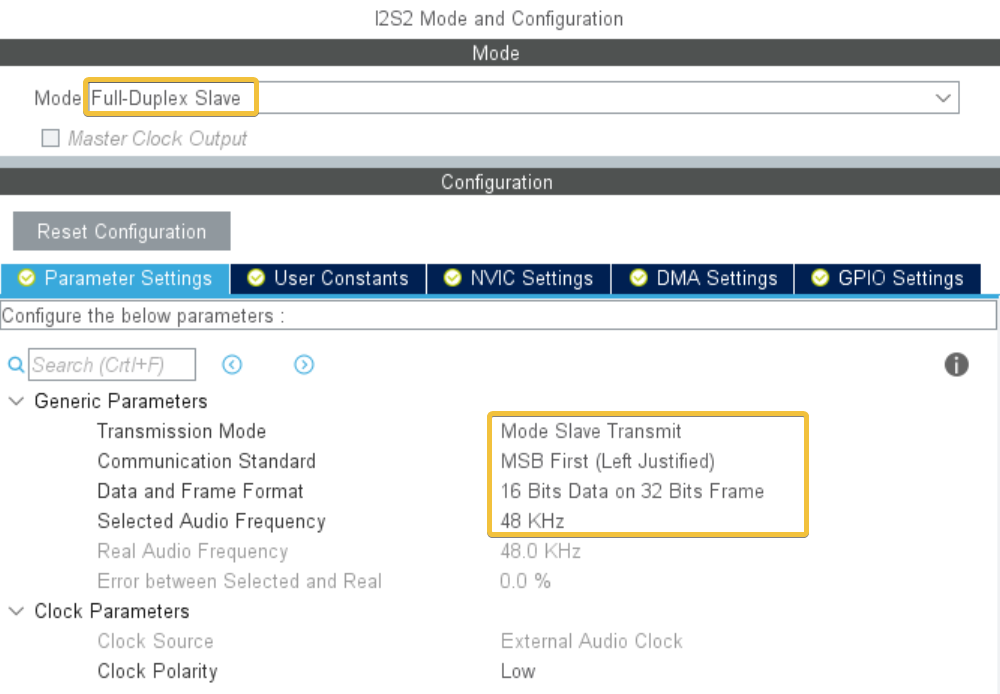
\includegraphics[width=0.9\linewidth]{CubeMX_I2S}
	\caption{Parameter Einstellungen der I\textsuperscript{2}S2 Schnittstelle}
	\label{pic:CubeMX_I2S}
\end{figure}

Da der TLV320 Codec im Master Modus betrieben wird, ist der STM32 im \\
\texttt{Mode Slave Transmit}.
Auch die Justification und die Wortbreite muss mit dem TLV320 übereinstimmen. Hier wird \texttt{MSB First} mit 16 Bits auf einem 32 Bit Frame eingestellt.
Die Samplingrate beträgt $f_s = 48\si{kHz}$.

Für die I\textsuperscript{2}S Schnittstelle wird die automatische Datenübertragung mittels DMA verwendet. Die Konfiguration des DMA Controllers ist in Abschnitt \ref{sec:CubeMXDMA} beschrieben.

